\documentclass[11pt,a4paper]{article}

% ---------- Packages ----------
\usepackage[utf8]{inputenc}
\usepackage[T1]{fontenc}
\usepackage{lmodern}
\usepackage{geometry}
\usepackage{float}
\usepackage{placeins}
\usepackage{caption}
\geometry{margin=1in}
\usepackage{setspace}
\onehalfspacing
\usepackage{graphicx}
\usepackage{hyperref}
\usepackage{csquotes}
\usepackage{enumerate}
\usepackage{xcolor}
\usepackage{listings}
\usepackage[style=authoryear,maxcitenames=2,backend=biber]{biblatex}

% ---------- Listings configuration for code highlighting ----------
\definecolor{codegreen}{rgb}{0,0.6,0}
\definecolor{codegray}{rgb}{0.5,0.5,0.5}
\definecolor{codepurple}{rgb}{0.58,0,0.82}
\definecolor{backcolour}{rgb}{0.95,0.95,0.95}

\lstdefinestyle{soliditystyle}{
    backgroundcolor=\color{backcolour},
    commentstyle=\color{codegreen},
    keywordstyle=\color{blue},
    numberstyle=\tiny\color{codegray},
    stringstyle=\color{codepurple},
    basicstyle=\ttfamily\footnotesize,
    breakatwhitespace=false,
    breaklines=true,
    captionpos=b,
    keepspaces=true,
    numbers=left,
    numbersep=5pt,
    showspaces=false,
    showstringspaces=false,
    showtabs=false,
    tabsize=2,
    frame=single,
    morekeywords={contract,function,public,private,external,internal,view,pure,returns,return,
                  address,uint256,uint,int256,int,bool,bytes,string,mapping,struct,enum,
                  modifier,event,require,assert,revert,if,else,for,while,constructor,
                  indexed,emit,payable,memory,storage,calldata,immutable}
}

% ---------- Bibliography file ----------
\addbibresource{references.bib}

% ---------- Title ----------
\title{\textbf{The Rainy-Day Fund: Decentralized Parametric Insurance for Smallholder Farmers in Kenya}}
\author{
	Group A: Ellena, Sabina, Noah, Vincent\\[0.5em]
	\textit{University of Basel, Blockchain Challenge 25}
	}
	\date{\today}

	% ---------- Section formatting and ToC ----------
	\usepackage{titlesec}
	\usepackage{tocloft}
	\setcounter{secnumdepth}{3}
	\setcounter{tocdepth}{2}
	\titleformat{\section}
	{\Large\bfseries}{\thesection}{1em}{}
	\titlespacing*{\section}{0pt}{2.0ex plus .2ex minus .2ex}{1.0ex plus .2ex}
	\titleformat{\subsection}
	{\large\bfseries}{\thesubsection}{1em}{}
	\titlespacing*{\subsection}{0pt}{1.5ex plus .2ex minus .2ex}{0.8ex plus .2ex}
	\renewcommand{\cftsecfont}{\normalfont}
	\renewcommand{\cftsubsecfont}{\normalfont}
	\renewcommand{\cftsecpagefont}{\normalfont}
	\setlength{\cftbeforesecskip}{4pt}

	\begin{document}
	\maketitle

	\begin{abstract}
    Smallholder farmers in Kenya face serious challenges due to climate variability, as more than 98\% of agriculture depends on rain-fed systems and much of the country's arable land lies in arid and semi-arid regions (ASALs).
    Frequent droughts, unpredictable rainfall, and extreme weather events have reduced crop yields, threatened food security, and put rural livelihoods at risk.
    Traditional risk mitigation strategies, including crop diversification and off-farm income, remain insufficient, while irrigation development is limited due to infrastructural and environmental constraints.
    Weather index insurance (WII) has emerged as a practical solution because it provides affordable, quick, and reliable payouts based on objective weather data, while reducing administrative costs and moral hazard.
    Building on this idea, the Rainy-Day Fund introduces a decentralized, blockchain-based parametric insurance system.
    By using smart contracts and mobile payment platforms, it can deliver timely payouts to farmers, strengthen their resilience, and help them reinvest in their farms.
    This approach not only protects farmers from the financial shocks of extreme weather but also offers a transparent and efficient way to support sustainable agricultural livelihoods.
    \end{abstract}

    \textbf{Keywords:} Smallholder farmers, Kenya, climate change, weather index insurance, parametric insurance, blockchain, agricultural resilience, arid and semi-arid lands.

    % Table of Contents
    \tableofcontents
    \bigskip

    \section{Goals and Motivation}\label{sec:goals}
    The goal of the Rainy Day Fund is to design a decentralized parametric insurance solution that can provide smallholder farmers with affordable, fast, and trustworthy protection against climate-related risks.
    By leveraging blockchain technology, the project seeks to overcome mistrust, high administrative costs, and inefficiencies that have limited adoption of weather index insurance.
    The motivation lies in addressing urgent climate vulnerabilities, reducing poverty traps, and creating scalable financial safety nets in one of the world's most underserved insurance markets.

    \section{Introduction}\label{sec:intro}
    Agriculture is the backbone of Kenya's economy, contributing approximately 21.3\% to the country's GDP in 2024~\parencite{WorldBank2024}.
    It is the largest employer in the country, providing livelihoods for over 40\% of the total population and more than 70\% of the rural population~\parencite{FAO2024}.
    Smallholder farmers form the majority of agricultural producers, yet they remain highly vulnerable to climate variability.

    Kenya's Arid and Semi-Arid Lands (ASALs) cover about 89\% of the country's land area, host over 70\% of livestock, and are home to around 36\% of the population~\parencite{IUCN, NDMA2021, UNEP-DHI}.
    Farmers in these regions depend almost entirely on rain-fed crops and livestock, making them extremely vulnerable to droughts and erratic rainfall.
    The drought between 2020 and 2023, the worst in four decades, illustrates the severity of this risk as farmers faced severe yield losses in many regions, 2.6 million livestock were lost, and 4.4 million people required urgent food assistance~\parencite{TheStar2024, NationalDroughtManagementAuthority2024}.

    These shocks highlight the fragility of rural livelihoods and the absence of effective financial safety nets to protect farmers.
    This paper proposes a decentralized, blockchain-based parametric insurance model as a potential solution to bridge this gap.
    Our guiding research question is: How can blockchain-based weather insurance provide affordable, transparent, and automatic protection for rural farmers in Africa who are exposed to increasing climate risks?

    \section{Problem Analysis}\label{sec:problem}
    Smallholder farmers in Kenya are uniquely vulnerable to climate risks.
    About 98\% of Kenya's agricultural systems are rain-fed~\parencite{GovernmentOfKenya2017}, while irrigation development is limited due to infrastructural and environmental constraints~\parencite{Wairimu}.
    Traditional coping strategies such as crop diversification, off-farm work, and borrowing are insufficient to withstand the growing severity of climate shocks.
    As a result, households often fall into poverty traps, selling livestock or assets after droughts and struggling to recover in later seasons.
    The drought between 2020 and 2023, considered the worst in four decades, illustrates the magnitude of the challenge as farmers experienced severe yield losses in affected areas, more than 2.6 million livestock died, and about 4.4 million people required urgent food assistance~\parencite{OCHA2023}.
    These shocks do not only affect farmers individually but also ripple across Kenya's economy, since agriculture contributes over 20\% of national GDP and supports the majority of rural livelihoods~\parencite{WorldBank2024}.

    Conventional agricultural insurance is largely absent in Kenya, and where it does exist, it suffers from deep structural weaknesses.
    High administrative costs make premiums unaffordable for smallholder farmers~\parencite{DominguezAnguianoParte2024}.
    Claims are processed slowly and often manually, which delays payouts and worsens farmers' financial stress during crises~\parencite{Chainlink2021}.
    A lack of transparency around pricing and claims fosters mistrust~\parencite{DominguezAnguianoParte2024}.
    Moreover, coverage remains minimal, as fewer than 3\% of farmers in Sub-Saharan Africa are insured, leaving more than 97\% unprotected~\parencite{WorldBank2022}.

    Weather Index Insurance (WII) has emerged as a potential tool to address these challenges, because it relies on measurable weather data such as rainfall or temperature thresholds to trigger payouts.
    This reduces delays, administrative costs, and moral hazard compared to traditional indemnity-based insurance~\parencite{Jensen2016, Sibiko2018}.
    Studies show that WII adoption can reduce poverty, improve household welfare, and encourage investment in improved seeds and fertilizers.
    Yet despite this potential, uptake remains very limited.
    Farmers often lack awareness or financial literacy, making WII appear too complex~\parencite{Janzen2020}.
    Basis risk remains a major concern, as mismatches between weather station data and on-farm realities can result in payouts that do not reflect actual losses, undermining trust~\parencite{Jensen2016}.
    Affordability is another barrier, since many farmers lack liquidity at the beginning of the planting season, precisely when premiums are due.

    These systemic shortcomings are reflected in the lived experiences of farmers like \textit{Mary}, a 38-year-old smallholder living in a semi-arid region of Kenya.
    Mary is married with three children and owns a basic Android phone, but she has no formal insurance.
    For her, every drought threatens both her harvest and her household income.
    When she does consider insurance, she struggles to afford premiums upfront, finds products too complex to understand, and doubts that payouts would be delivered fairly or on time.
    Even if she were to purchase a policy, she fears that unreliable weather data would not capture the realities of her farm.
    As she puts it, \enquote{Why should I pay if they don't measure my reality?}
    Mary's skepticism mirrors the sentiments of millions of smallholder farmers across Kenya who remain excluded from meaningful risk protection.

    \section{Benefits of Blockchain in Insurance}\label{sec:benefits}

    \subsection{Blockchain \& Decentralized Microinsurance}\label{subsec:blockchain-&-decentralized-microinsurance}
    Blockchain technology, with its decentralized ledger and automated smart contracts, is particularly well-suited for microinsurance solutions targeting smallholder farmers.
    By eliminating intermediaries, automating claims, and ensuring transparency, blockchain can reduce operational costs, increase trust, and make insurance accessible even in remote areas~\parencite{DominguezAnguianoParte2024, Shetty2022}.
    Moreover, parametric microinsurance, where payouts are triggered by measurable weather events, benefits from blockchain's immutable and auditable infrastructure, ensuring rapid and verifiable payments.
    Despite early adoption challenges, integrating blockchain into agricultural insurance provides a scalable, efficient, and reliable solution to climate risk, bridging gaps in coverage for underserved populations.

    \subsection{Problems with Traditional Insurance}\label{subsec:problems-with-traditional-insurance}
    Traditional insurance faces several critical challenges that limit its effectiveness, particularly in agricultural and microinsurance contexts.
    Transparency is often lacking, so policyholders cannot easily see how premiums are set, how claims are assessed, or why payouts are delayed.
    This lack of clarity fosters distrust between insurers and customers~\parencite{DominguezAnguianoParte2024}.
    Claims are also slow and mostly manual, requiring extensive paperwork and human assessment.
    These delays can worsen farmers' financial stress during climate shocks~\parencite{Chainlink2021, Shetty2022}.
    High administrative costs associated with record-keeping, fraud checks, and staffing are often passed on as expensive premiums, making insurance unaffordable for smallholder farmers~\parencite{DominguezAnguianoParte2024}.
    The reliance on self-reported or incomplete data further raises the risk of fraud and moral hazard, while detecting and preventing fraud requires significant resources~\parencite{Chainlink2021, Shetty2022}.
    Finally, coverage remains extremely limited.
    In Sub-Saharan Africa, less than 3\% of farmers are insured due to logistical, financial, and trust barriers, and the centralized structure of traditional insurance often makes it difficult for rural farmers to access services~\parencite{Alsdorf2024, WorldBank2022}.

    \subsection{Blockchain Advantages}\label{subsec:blockchain-advantages}
    Blockchain technology helps address many of the weaknesses in traditional insurance by providing a decentralized, tamper-proof ledger that builds transparency and trust without relying on a central authority~\parencite{Shetty2022}.
    Smart contracts can automate claims and payouts, reducing the need for human involvement and lowering administrative costs~\parencite{Chainlink2021, DominguezAnguianoParte2024}.
    Because records on the blockchain are immutable, they cannot be tampered with, which prevents fraudulent claims.
    Decentralized oracles also supply reliable and verifiable data for triggering insurance events.
    In addition, blockchain can connect easily with mobile wallets, allowing farmers in remote or underserved areas to access insurance services directly~\parencite{DominguezAnguianoParte2024}.

    \subsection{Benefits for Parametric \& Microinsurance}\label{subsec:benefits-for-parametric-&-microinsurance}
    Applying blockchain to parametric insurance enables fully automated, event-based payouts, reducing basis risk, enhancing speed, and improving trust among stakeholders~\parencite{Chainlink2021, ParametricInsured2025, Shetty2022}.
    For microinsurance, blockchain improves cost efficiency by lowering policy management costs, making it possible to expand coverage to underserved farmers and to explore flexible pricing models~\parencite{DominguezAnguianoParte2024, ResearchGate2023}.
    Real-world examples such as Etherisc and Arbol already show how this can work in practice, with thousands of farmers receiving instant payouts without the need for manual claims assessments~\parencite{Alsdorf2024, DominguezAnguianoParte2024, ParametricInsured2025}.
    The combination of decentralization, automation, and verifiable data ensures that parametric microinsurance is transparent, scalable, and trustworthy~\parencite{Shetty2022}.

    \section{Target Market \& Stakeholders}\label{sec:targetmarket}
    Smallholder farmers in Kenya, particularly those living in the Arid and Semi-Arid Lands (ASALs), represent the primary target market for decentralized parametric insurance.
    These regions cover about 89\% of the country's land area, host over 70\% of the livestock population, and are home to roughly 36\% of the national population~\parencite{IUCN, NDMA2021, UNEP-DHI}.
    With more than 98\% of agriculture dependent on rain-fed systems, smallholder farmers are disproportionately exposed to climate variability and shocks~\parencite{GovernmentOfKenya2017}.
    Agriculture employs around 40\% of Kenya's total population and over 70\% of the rural population, yet fewer than 1\% of farmers currently purchase agricultural insurance, leaving the vast majority unprotected~\parencite{FAO2024, MinistryOfAgriculture2023}.

    The stakeholders in Kenya's agricultural insurance ecosystem are diverse and interdependent.
    Farmers are the primary end-users, seeking affordable and trustworthy protection against climate risks.
    Insurers and micro-insurers, such as APA Insurance, UAP, CIC, Jubilee, and Kenya Orient, underwrite and distribute weather-index products, while global reinsurers like Swiss Re provide the financial backing needed for large-scale coverage~\parencite{Artemis2017, BASIS2017}.
    The Government of Kenya, through its National Agricultural Insurance Policy (NAIP), and regulatory agencies such as the Insurance Regulatory Authority (IRA) and the National Drought Management Authority (NDMA), sets regulations and coordinates drought response~\parencite{AfricanClimateFoundation2024, MinistryOfAgriculture2023}.
    International donors and development partners, including the World Bank, IFC, and FAO, subsidize premiums, and provide technical support, as seen in the Kenya Livestock Insurance Program (KLIP)~\parencite{Artemis2017, WorldBank2022}.
    Finally, mobile money services such as Safaricom's M-Pesa make it possible to collect premiums and deliver payouts directly to farmers~\parencite{OxfordBusinessGroup2017}.

    \section{Market Research \& Competitor Analysis}\label{sec:marketresearch}
    Agricultural insurance penetration in Kenya remains extremely low, even though agriculture forms the backbone of the economy.
    The Government's National Agricultural Insurance Policy (NAIP) highlights that less than 1\% of farmers and pastoralists purchase agricultural insurance, leaving the vast majority of producers exposed to climate shocks without any formal safety net~\parencite{MinistryOfAgriculture2023}.
    Across Sub-Saharan Africa, the picture is similar.
    There are about 48 million smallholder farmers, yet fewer than 1.5 million are insured.
    This means that only around 3\% have coverage, leaving 97\% unprotected, despite an annual demand estimated at USD 10--14 billion compared to a premium pool of only USD 1--3 billion~\parencite{ACREAfrica2020}.
    These figures highlight an enormous protection gap, both in Kenya and across the region, where millions of rural households face severe climate risks without reliable financial buffers.

    Despite these low figures, recent pilots suggest that demand exists when products are designed to be affordable, transparent, and accessible.
    For instance, the World Bank–supported One Million Farmers Platform has enabled over 70,000 smallholders across 15 counties to access weather-index insurance, primarily through digital delivery channels and bundled products.
    This suggests that the barrier is not farmer willingness but the way insurance is designed and distributed~\parencite{WorldBank2022}.

    On the supply side, Kenya already offers both livestock and crop index solutions.
    The Kenya Livestock Insurance Program (KLIP) is a leading public--private partnership providing drought insurance in ASAL counties.
    It is run by a consortium of local insurers led by APA (together with UAP, CIC, Jubilee, Heritage, Amaco, and Kenya Orient) and supported by Swiss Re as reinsurer.
    KLIP has successfully delivered multi-million-shilling payouts when drought thresholds were met~\parencite{Artemis2017, BASIS2017}.
    KLIP demonstrates proof of concept for index insurance in Kenya, showing that government support, consortium underwriting, and reinsurer participation can combine to deliver payouts at scale.

    In the crop sector, ACRE Africa and Pula are the leading intermediaries.
    ACRE Africa has developed weather-index products that are increasingly bundled with agronomic services, such as advisory tools and crop-cutting experiments, to improve product value and data accuracy~\parencite{ACREAfrica2024}.
    Pula, by contrast, has built scale across Africa by bundling insurance with seeds, fertilizer, and other farm inputs, often distributed through governments and value-chain partners.
    Its use of satellite and remote sensing data has enabled broad coverage, though it continues to face challenges with basis risk and farmer liquidity constraints at planting~\parencite{MunichReFoundation2022, UNSGSA2023}.

    More recently, blockchain-based models have entered the Kenyan market.
    Etherisc, in collaboration with ACRE Africa, piloted a \enquote{Bima Pima} crop cover in 2021, reaching over 17,000 farmers and delivering the first blockchain-based payouts in Kenya.
    By embedding smart contracts and decentralized oracles into the insurance process, Etherisc was able to automate claim settlement and reduce administrative overhead~\parencite{Etherisc2021}.
    Although small in scale, this pilot shows how blockchain can help reduce long-standing problems in agricultural insurance, especially those related to trust, transparency, and timely payouts.

    OKO Finance, for example, has demonstrated in Mali and Uganda how mobile-first, index-based agriculture insurance can be structured using satellite or remote sensing data and delivered through digital channels~\parencite{ADA_OKOFinance2021}.
    Although OKO is not known to be active in Kenya at the moment, its model suggests how digital ecosystems could lower distribution costs and expand access to underserved farming populations.

    In short, agricultural insurance in Kenya is still underdeveloped, with less than 1\% of farmers insured.
    However, programs like KLIP and private-sector innovators such as ACRE Africa and Pula show that growth is possible.
    Farmers still face major barriers, including basis risk~\parencite{Jensen2016}, limited awareness and perceived complexity~\parencite{Janzen2020}, and upfront liquidity constraints all reduce trust and limit uptake.
    Early blockchain pilots such as Etherisc's indicate promising pathways to reduce administrative costs and improve transparency, but scaling such solutions will depend on robust data infrastructure, effective oracles, and farmer-centric design.
    Overall, the market reflects both a large protection gap and a significant opportunity, as innovative, technology-enabled models that combine affordability, transparency, and mobile integration have the potential to transform risk management for Kenya's smallholder farmers.	

\section{Solution Design}\label{sec:solution design}

\subsection{Business Model}

\subsubsection{Overview}
The Rainy Day Fund is a two-sided parametric insurance marketplace. Farmers obtain seasonal drought protection through ERC-20 policy tokens, while investors provide liquidity to an ERC-4626 vault and receive proportional shares. A smart contract manages issuance, pooling and payouts. The design reduces administrative overhead and shifts pricing and risk allocation to a market-based mechanism.

\subsubsection{Problem and Customer Segments}
Smallholder farmers in Kenya face recurrent rainfall shocks but lack access to formal insurance. High distribution costs, weak trust in insurersan d limited actuarial data block traditional coverage. At the same time, impact-oriented investors seek transparent, uncorrelated instruments. The marketplace connects both groups, while cooperatives, NGOs and telcos provide distribution and trust infrastructure ~\parencite{cole2013barriers}.

\subsubsection{Value Propositions}
\begin{itemize}
    \item \textbf{Farmers}: affordable coverage, predictable payouts triggered by rainfall indices, and mobile transactions via M-Pesa.
    \item \textbf{Investors}: standardized exposure to agricultural risk with measurable yield, diversifying traditional portfolios.
    \item \textbf{Partners}: reduced leakage and transparent performance metrics for evaluation and reporting.
\end{itemize}

\subsubsection{Solution Design}
Farmers purchase ERC-20 tokens as digital proof of coverage. Investors deposit capital into an ERC-4626 vault and receive fungible shares. Oracle-based rainfall indices determine payout eligibility. Premiums and yields are set through a seasonal sealed-bid uniform-price auction functioning as a prediction market: farmer bids and investor offers jointly reveal the market-implied drought probability $\hat{\pi}$ and equilibrium margin \citep{hanson2003market,wolfers2004prediction}. The frontend abstracts blockchain logic and integrates fiat--stablecoin conversion.

\subsubsection{Revenue Model}
Premiums collected from farmers fund the risk pool. Investor returns correspond to the surplus of premiums over payouts, distributed proportionally through vault shares. The auction internalizes both risk expectations and operational costs into the equilibrium premium, creating endogenous funding for the platform.

The operator may also allocate its own capital into the pool. This dual role enhances credibility and creates an additional revenue stream if claims remain below expectations, though it increases exposure to volatility. A 2--5\% operator fee on premiums covers infrastructure, audits, and compliance. Optional reinsurance transfers catastrophic risk to external providers and stabilizes investor yields ~\parencite{cummins2009catastrophe}.

ERC-4626 shares accumulate value as premiums flow in and payouts are deducted. Because surpluses are automatically reinvested into vault NAV, long-term investors experience a compounding effect similar to conventional finance. Payouts are not broadcasted indiscriminately; they require a minimal on-chain claim, after which the contract settles automatically if the rainfall index threshold is breached (see Claim Process and Payout Logic).

\subsubsection{Cost Structure}
Key cost drivers are oracle services, secure data feeds, system audits, regulatory engagement, payment integration, and farmer outreach. Automation keeps administrative costs lower than in conventional microinsurance. Economies of scale further reduce marginal costs as the pool and user base expand.

\subsubsection{Channels and Partnerships}
Cooperatives, NGOs, and agro-dealers provide farmer onboarding and trust. M-Pesa integration allows direct premium and payout transactions. Oracle providers deliver rainfall indices ~\parencite{egberts2017oracle}. Reinsurers supply capacity for tail risk. Regulators and development agencies support compliance and market acceptance.

\subsubsection{Scalability}
The model can expand from Kenyan maize to other crops, regions, and perils such as livestock mortality or flood. ERC standards allow interoperability with DeFi protocols and secondary markets for risk exposure. The prediction-market mechanism improves with scale, as more participants and data sources sharpen price discovery. Modular system design supports adjustments across regulatory environments.

\subsubsection{Claim Process and Payout Logic}
Farmers must file a minimal on-chain claim (notice-of-loss) during a specified window $[t_0,t_1]$ after oracle publication. The contract verifies:
\begin{enumerate}
    \item ownership: policy tokens $q>0$ for the epoch,
    \item uniqueness: no prior claim from the same address/epoch,
    \item eligibility: oracle index $I$ satisfies $I \le \tau$.
\end{enumerate}
If (1)--(3) hold, the contract transfers $qL$ (or pro-rata if rationing applies) from the vault to the claimant’s wallet; otherwise the call reverts. Operational costs $F$ are deducted before distribution. No off-chain adjusters or discretionary assessments occur.\footnote{A claim call is required to (i) prevent automatic transfers to inactive or lost wallets, (ii) avoid dust payouts below gas costs, and (iii) let farmers select their preferred payout rail (e.g. M-Pesa bridge).}

\section{Mechanism Design}\label{sec:mechanism design}

Premiums and investor yields are discovered through a pre-season sealed-bid uniform-price auction. This single mechanism acts as a prediction market for drought risk, while remaining implementable under smallholder constraints ~\parencite{wilson1979auctions,ausubel2002demand}.  

\subsubsection{Notation}

Let $x$ denote the number of insurance tokens sold, with $Q$ referring to the total seasonal quantity (so $Q=x$ at equilibrium). Each token promises a payout $L$ if drought occurs, represented by the indicator variable $X \in \{0,1\}$. Farmers pay a premium $p$ per token.  

We define $\hat{\pi}$ as the \emph{market-implied probability of drought}, inferred endogenously from the auction clearing. Premiums decompose into $\hat{\pi}L$ and the risk margin $\mu$. Operational costs are $F$, investor capital $K$, realized return $R$, and expected return $R^\star$. Farmer inverse demand is $p_d(x)$; investor supply is $C_s(R)$. Required reserves are $C_{\mathrm{req}}(x)$, with prudential utilization factor $\theta \in (0,1]$.  

\subsubsection{Auction Process and Clearing Mechanism}

At the beginning of each season, farmers submit bids $(q_i, p_i)$ and investors submit $(k_j, R_j)$. Bids are committed via a commit--reveal protocol ~\parencite{blum1983coinflipping,buterin2015commit,parkes2014mechanism}, ensuring confidentiality until revelation.  

Feasibility requires
\[
C_{\mathrm{req}}(x) = xL\theta \leq S(R), \quad x \leq D(p).
\]
Expected return for coverage $x$ at premium $p$ is
\[
R = \frac{px - \hat{\pi}xL - F}{K}.
\]

The mechanism adopts the \emph{full coverage rule}: clearing at the maximal feasible $x^\ast$. The clearing premium is
\[
p^\ast = \min\{p_i : \sum_i q_i \geq x^\ast\},
\]
and the corresponding expected return $R^\ast$ follows from the cashflow identity. All accepted farmer bids pay $p^\ast$, all investor capital earns $R^\ast$. If demand exceeds feasible coverage, allocations are scaled proportionally:
\[
q_i^{\text{alloc}} = \rho q_i, \qquad \rho = \frac{x^\ast}{\sum_i q_i}.
\]

\subsubsection{Premium Decomposition and the Risk Margin}

The clearing premium decomposes into expected actuarial loss and a margin:
\[
p = \hat{\pi}L + \mu.
\]

Investor cashflow is
\[
CF = pQ - XQL - F,
\]
with realized return
\[
R = \frac{CF}{K}, \quad
R^\star = \frac{pQ - \hat{\pi}QL - F}{K}.
\]

It follows that
\[
\mu = \frac{R^\star K + F}{Q}.
\]

Operational costs $F$ are deducted transparently by the contract before distribution. They reduce net cashflows, but investors anticipate them when bidding \citep{bowers1997actuarial}.

\subsubsection{Joint Market Equilibrium}

Auction outcomes satisfy equilibrium conditions:
\[
p^\ast = p_d(x^\ast), \qquad C_s(R^\ast) = C_{\mathrm{req}}(x^\ast).
\]

For analysis, demand is approximated by an isoelastic form \citep{mascolell1995microeconomic,varian1992micro}:
\[
p_d(x) = A x^{-1/\varepsilon}, \quad \varepsilon > 0,
\]
and supply linearly:
\[
C_s(R) = a + bR, \quad b > 0.
\]  

Seasonal outcomes $(Q,p)$ are then fitted ex post with a convex bonding curve:
\[
p(x) = \max\!\left(p_{\min},\, p_{\min}\Big(1+\frac{\lambda x}{N}\Big)^k\right),
\]
providing a tractable approximation for forecasting \citep{angeris2020improved,shiller2003bond}. This curve is used \emph{only for analysis}, not for live pricing.

\subsubsection{Allocation Rules and Fairness}

Pro-rata rationing ensures envy-freeness when demand exceeds feasible capacity:
\[
q_i^{\text{alloc}} = \rho q_i, \qquad \rho = \frac{\bar{Q}}{\sum q_i}.
\]

Alternative rules (cutoffs, discriminatory allocations, priority mechanisms) were rejected as less efficient or less fair. Full coverage with pro-rata allocation mobilizes all feasible capacity while minimizing envy.

\subsubsection{Limitations and Future Research}

Limitations remain. Functional forms for demand, supply and bonding curves require calibration. $\hat{\pi}$ must be validated against external actuarial or climate models. Uniform-price auctions remain vulnerable to demand reduction. Commit--reveal protocols face risks of collusion or non-reveal failures. Finally, convex pricing could disadvantage liquidity-constrained farmers. Future research should calibrate with field data, add anti-collusion safeguards and test continuous models as counterfactuals.

	
	\section{Implementation}\label{sec:implementation}
	Overview of implementation goals, strategy and architecture.

	The goal for this project was providing a showcase prototype .
	Therefore, the focus was on providing the most important features, a neat, easy UI and a good test-setup to showcase the functionality and laying the groundwork for possible extensions.
	These extensions and some of the more advanced features that were not provided in the prototype will be discussed in sections~\ref{subsec:qa-security} and~\ref{subsec:outlook}
	It is important to note that the project is not a complete MVP (minimum viable product), due to the constraints when it comes to funding for example Chainlink as provider for weather data or using actual currency as a payment method.


	\subsection{Development Process \& Strategy}\label{subsec:dev-strategy}
	The strategy for the implementation was largely based on a learning process.
	At first the focus was mainly on exploring the basics of Solidity based Smart Contracts and creating an early working prototype.
	Once this was achieved the focus shifted to code quality, finding efficient and well established solutions to tackle current challenges and at the end, integrating all of this into an easy-to-use UI .


	The most important guidelines and ideas for the implementation were:

	\begin{enumerate}[1]
		\item \textbf{Division of Work:} The work was divided mostly into two parts.
			One part was the overarching architecture and product design, including specifically the smart contract development using Solidity, as well as researching existing libraries and standards to implement and use.
			The other part, equally important was researching and setting up the tools and frameworks for everything else: The project and testing setup using Hardhat and writing the actual test-code, implementing the UI, using React, Managing the Repository, and bug-fixing.
			This division was important for numerous reasons, but especially because it allowed for mutual verification and simultaneously the possibility to truly focus on specific topics.
		\item \textbf{Testing Setup:} The Testing-Setup within Hardhat and using Node.js made finding bugs and testing after changes much more efficient and also allows for neat and compact showcases of the features and working prototype code.
			An excerpt from this testing setup and what it shows can be seen in figure~\ref{fig:test-set-up}.
		\item \textbf{Research:} Research was an important, continuous process throughout the project, for finding technical solutions but also possible issues with the current state of the project.
		\item \textbf{Usage of AI:} AI was used throughout the project for research purposes, when trying to find fitting libraries, tools and standards, as well as making repetitive tasks, like writing test code more efficient.
	\end{enumerate}

	An important challenge was to align technical progress with the economic modeling.
	Once a working prototype was achieved, communication between these two distinct work streams came into focus.
	Daily synchronization and change management helped in finding ways to implement the most important parts of the business model, whilst simplifying other parts, like using a mock weather oracle, instead of Chainlink as a source of weather data.
	The strategy during the development process was to implement based on an objective hierarchy:

	\begin{enumerate}[1]
		\item Working Smart Contract with deterministic payouts
		\item Investment logic
		\item Investor incentive model (yield / compound interest)
		\item Tests and Code quality
		\item Working frontend for showcases and manual testing
		\item \ldots
	\end{enumerate}

	These are just the most important tasks that are included in the final prototype.
	For further necessary steps towards a finished product refer to~\ref{subsec:outlook}.


	\subsection{System (Macro) Architecture}\label{subsec:system-architecture}
	The macro architecture of the system is centered around the RainyDayFund smart contract, which acts as the core of the decentralized insurance platform.
	It is designed to be extensible for integration with oracles (such as Chainlink), \texttt{ERC20 tokens} as payment and is integrated within a frontend built with React.
	The architecture emphasizes modularity, and ease of use for both farmers and investors, as well as neat and easy testing and showcasing.

	\begin{figure}[H]
		\centering
		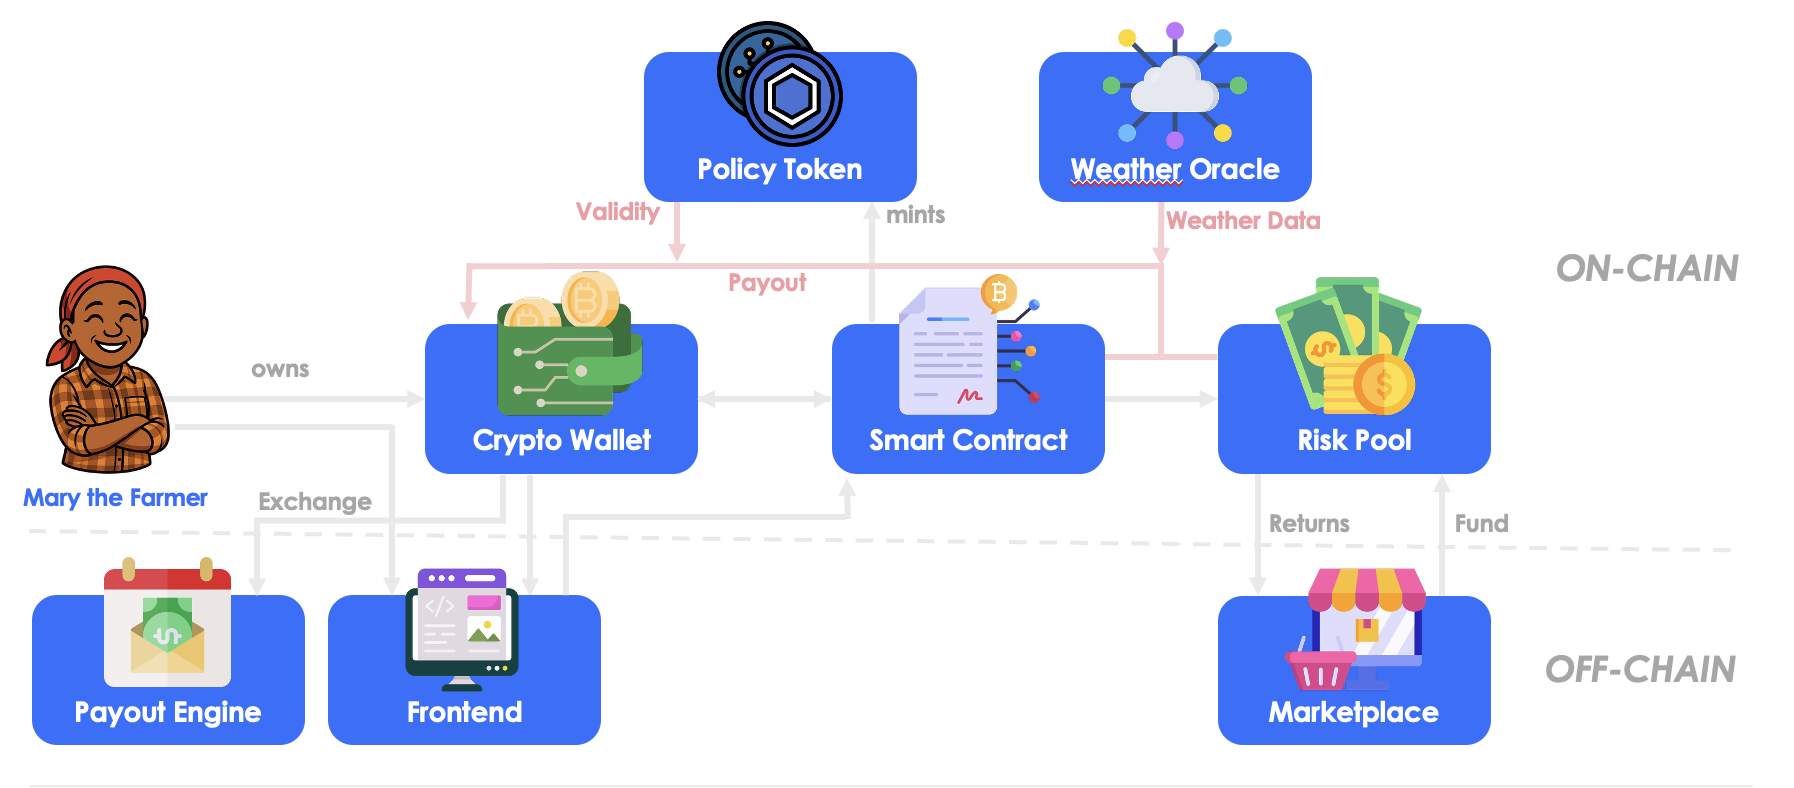
\includegraphics[scale=0.3]{graphics/Architectural_Overview}
		\caption{Architectural Overview \\ \textit{Source: Author's own.}}
		\label{fig:architecture}
	\end{figure}

	As shown in figure~\ref{fig:architecture} the users (both farmers and investors) own a crypto wallet and connect this to the frontend.
	The frontend then allows them to easily invest or buy policies for the current season with their crypto funds, by programmatically interacting with the Smart Contract.
	The smart contract then mints a policy token for farmers or deposits the investors funds in the vault, so that they can receive a yield.
	All funds are stored in a Risk-Pool (in our case the ERC4626 vault).
	The farmers can claim their policies at the end of the season and, if all conditions are met, i.e.\ the weather oracle gets and returns weather data, below the threshold and the farmer making the claim actually owns the policy tokens, receive their coverage funds.
	Investors may withdraw their funds, receiving all the accumulated yield.
	The \texttt{Payout Engine} symbolizes the possibility of transferring out funds from the crypto wallet to widely used mobile-money services, like M-Pesa.
	This is already a well established process and not included in the project itself, should however be noted, because it allows the farmers to actually immediately use their payouts in their everyday life.

	The concrete timeline for the process is based on the crop season and has 5 phases:
	\begin{enumerate}
		\item \textbf{Active Phase:} In the active phase policies can be bought and investments can be made.
			The premium for the current season is already set at the beginning through the auction-based system explained in section~\ref{sec:business-model} \textcolor{red}{check wether this links correctly!}.
			No claims or withdrawals can be made during this phase.
		\item \textbf{Inactive Phase:} Now the policies can no longer be bought, but investments can still be made.
			This allows for a speculative market for the insurance policies, while keeping the possibility of introducing more liquidity from capital investors.
		\item \textbf{Claim Phase:} The claim phase starts upon the actual crop season ending.
			Farmers may now try to claim their policies and receive their coverage payouts, while investors have to wait until this phase is over.
		\item \textbf{Withdrawal Phase:} Now investors may choose to withdraw their capital and receive their yield, while farmers wait until the next season is started.
		\item \textbf{Finished Phase:} The season is over, unclaimed policies are now invalid and not-withdrawn investments are used as liquidity for the next season, earning yield on the current investment (including the earned yield), creating a compounding effect.
        \label{enum:phases}
	\end{enumerate}


	\subsection{Smart Contract Design (Micro)}\label{subsec:smart-contract-design}
	The project is built around a Solidity smart contract using the Ethereum Virtual Machine.
	This central RainyDayFund contract can be called using the front end and holds all the exposed functionality for the consumer.
	Investors use the \texttt{invest()} and \texttt{withdraw()} methods while insurees can buy and claim their policies in batches using the \texttt{buyPolicy()} and \texttt{claimPolicies()} functions.
	The contract leverages the ERC1155 token standard for policy tokens, enabling efficient batch operations and flexible policy management.

	As shown in Figure~\ref{fig:initial-contract-design}, the initial contract made use of the \texttt{1155 token standard} for the \texttt{policyTokens}, to take advantage of the cost-efficient batch operations~\parencite{ERC1155}.
	To help with testing the (Mock)-MUSCD was created, implementing the ERC20 interface, to emulate the behavior of common stablecoins like USDC, which are used as payment and funding for the riskpool.
	This allowed for the free minting and full control over the coins and made testing the functionality of the main contract possible, even within the bounds of Remix VM .
	Therefore, testing was quicker and easier at the beginning, without the need to always deploy on the Sepolia Testnet or an immediate, complete setup, for example with hardhat.

	Initially there were multiple issues:
	\begin{enumerate}[1]
		\item \textbf{Mapping for storing addresses:} Initially we used a mapping to store who had bought policies and was thereby eligible to claim them.
			However, there were some issues with this: Firstly, the policies lost all their value when they were resold, because the address of the new owner would not be tracked in the mapping.
			Moreover, storing all of this data was very gas-inefficient and redundant, because ownership of the policyToken is proof of ownership for the policy.
		\item \textbf{No proper incentive for investors:} We had already planned to give the investors some incentive to keep their funds in the riskpool, even after the season would end, to increase liquidity for the next season.
			The idea to achieve this, was, to use compound interest or create some other form of yield over time.
			However, implementing this with the initial setup proved difficult and created vastly unfair results \textcolor{red}{Hier vllt nochmal genauer erkl\"aren}
		\item \textbf{Weather oracle:} The initial mock-up for the weather oracle was just a number that could be accessed and stored on the contract directly.
			This was far from the goal of using chainlink as a decentralized oracle to reliably and transparently access the data.
		\item \textbf{Attack vectors:} Lastly there were some attack-vectors, especially for the owner.
			The \texttt{startNewSeason()} function could be used at any point during the season, thus rendering unclaimed policyTokens worthless and not allowing for investment-withdrawals to be made.
	\end{enumerate}

	\begin{figure}[H]
		\centering
		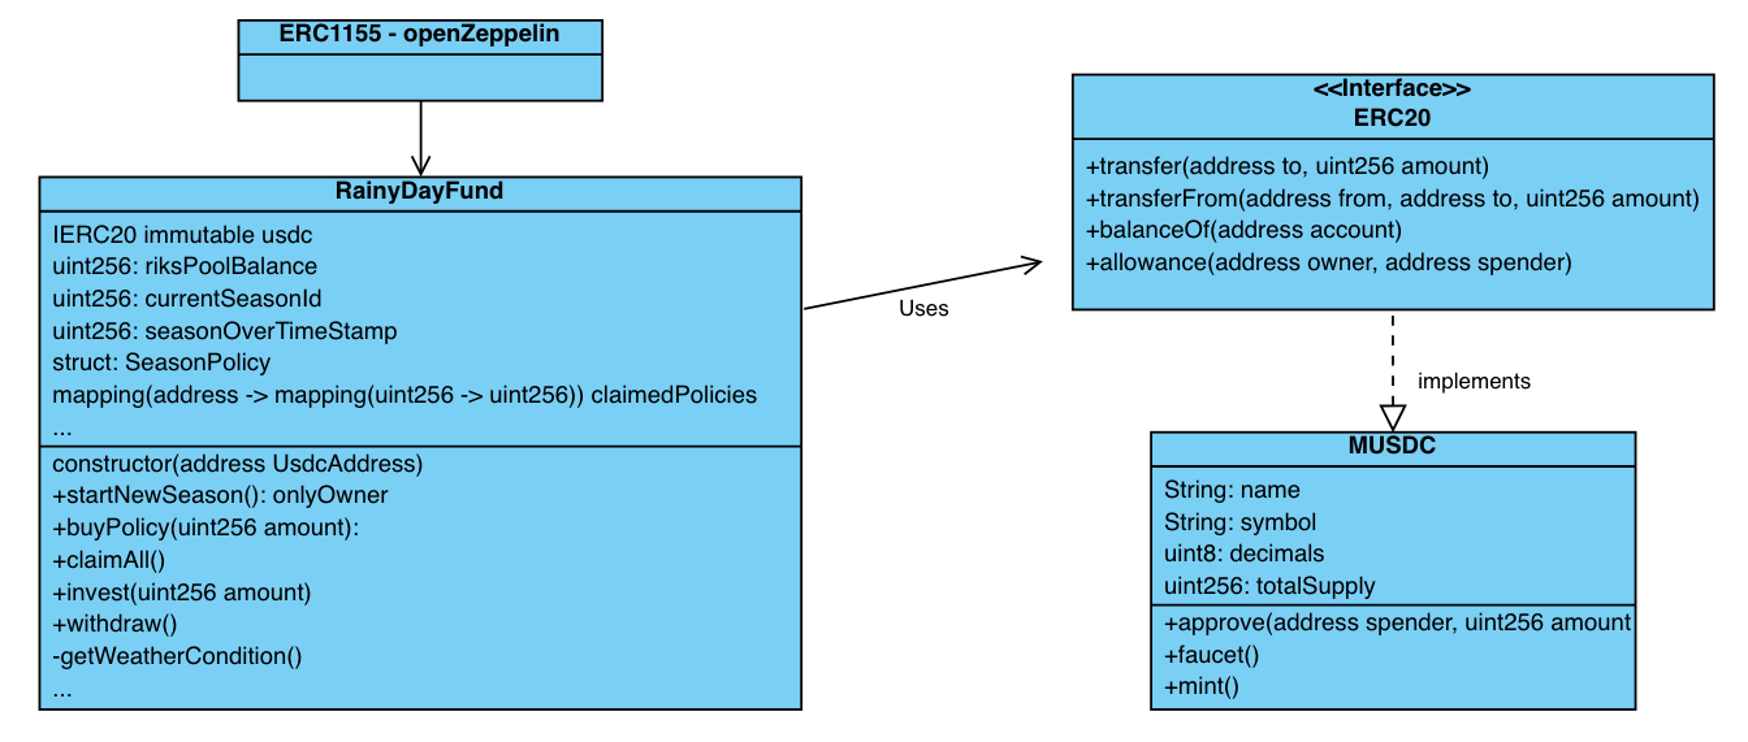
\includegraphics[scale=0.5]{graphics/ClassDiagram_Old}
		\caption{Initial Contract Design \\ \textit{Source: Author's own.}}
		\label{fig:initial-contract-design}
	\end{figure}

	Addressing these issues of the initial prototype the contract was restructured.
    The main fixes were:

    % Table: Major Issues and Fixes
    \begin{table}[H]
        \centering
        \caption{Major Issues and Corresponding Fixes}
        \label{tab:issues-fixes}
        \begin{tabular}{|p{0.42\textwidth}|p{0.42\textwidth}|}
            \hline
            \textbf{Issue} & \textbf{Fix} \\
            \hline
            Mapping for storing addresses was gas-inefficient and did not track policy resales & Removed the mapping \\
            \hline
            No proper incentive for investors and difficulties with implementation & Switched from self-made investment tracking to using the \texttt{ERC4626 vault} \\
            \hline
            Using Token Standards ERC4626, ERC20 and ERC1155 simultaneously, causing errors with inheritance of the contract & Switched from ERC1155 to only using ERC20 for the policyTokens \\
            \hline
            Weather Oracle / Chainlink integration & Implementing the proper Chainlink standards for the mock-up-weather oracle~\parencite{AggregatorV3Interface} \\
            \hline
            Attack Vector for Owner & Fixed some issues by including modifiers and properly implementing \enquote{mini-}state-machine (refer to enumeration~\ref{enum:phases}) \\
            \hline
        \end{tabular}
    \end{table}


    \subsection{Implementation: Final State of the project}\label{subsec:final-state}

    The final state of the contract can be seen here:

    \begin{figure}[H]
        \centering
        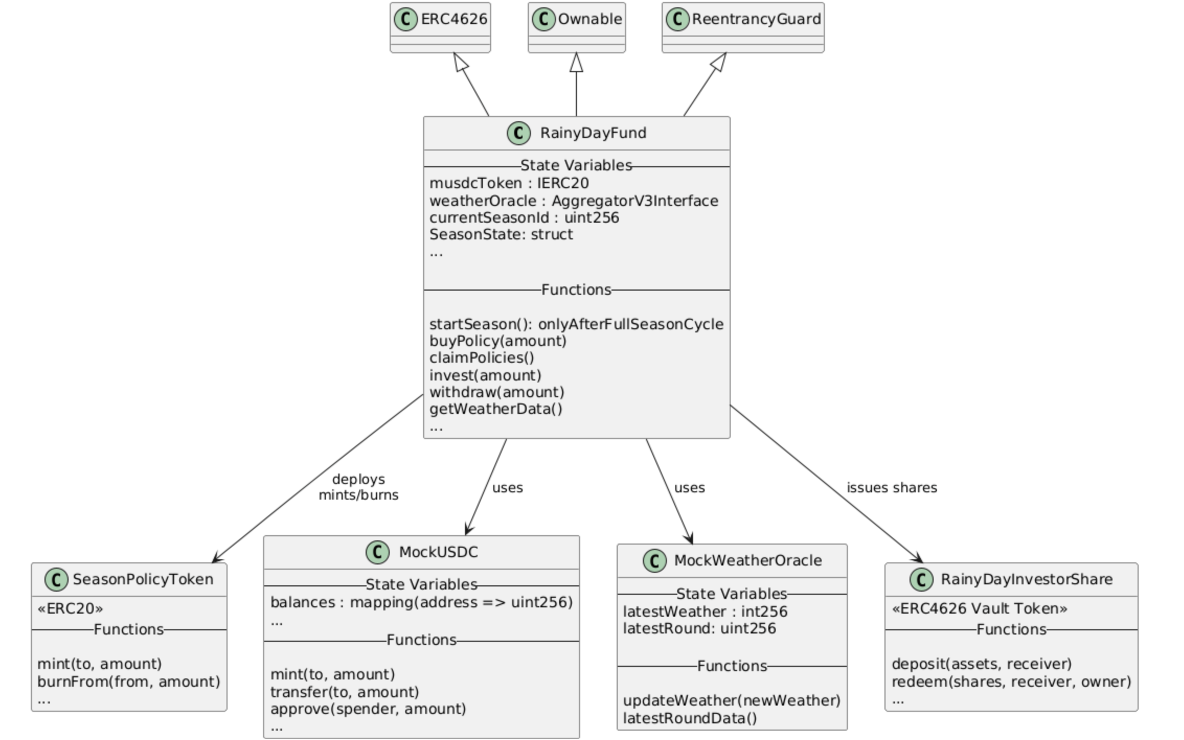
\includegraphics[scale=0.5]{graphics/ClassDiagram_New}
        \caption{Final Contract Design \\ \textit{Source: Author's own.}}
        \label{fig:final-contract-design}
    \end{figure}

    This class diagram only shows the most important functions and fields of the contract.
    The full code can be found in the appendix~\ref{sec:contract-code} along with some notes on its functionality.

    The constructor takes 2 arguments:
    \begin{enumerate}[(1)]
        \item \textbf{usdcAddress:} The address of the stablecoin that will be used for the transactions, here this would be the address of the deployed MockUSDC contract
        \item \textbf{weatherOracle:} The address of the weather data oracle service, here this would be the address of the deployed MockWeatherOracle contract, but in production should be the corresponding chainlink address.
    \end{enumerate}

    Both are required to not be zero and used to set the corresponding fields for further use.
    Then the first season is initialized.

    \begin{lstlisting}[style=soliditystyle, caption={RainyDayFund.sol - Main Insurance Contract},label={lst:lstlisting1}]
        ...

        constructor(address _usdcAddress, address _weatherOracle)
        ERC4626(IERC20Metadata(_usdcAddress))
        ERC20("RainyDay Investor Shares", "RDIS")
        Ownable(msg.sender)
            {
            require(_usdcAddress != address(0), "USDC address zero");
            usdc = IERC20(_usdcAddress);

            require(_weatherOracle != address(0), "Weather oracle zero");
            weatherFeed = AggregatorV3Interface(_weatherOracle);

            currentSeasonId = 1;
            _initializeSeason(currentSeasonId);
            seasonOverTimeStamp = getCurrentTime() + 2 * timeUnit;

            // Enable testing mode by default for local testing
            testingMode = true;
        }

        ...
    \end{lslisting}

    The contract utilizes a SeasonState enum to keep track of the phase that is currently active in the state Machine.
    The \texttt{getSeasonState()} method is used as the state machine and utilizes the \texttt{getCurrentTime()} method.
    The choice to implement the time this way, instead of simply using the \texttt{block.timestamp} was made to allow for time manipulation in testing.
    That is why there is a testingTimeOffset being added to the timestamp.
    This offset is calculated and set in a method of its own, that is only used for testing / showcasing reasons and would be removed for production.

    \begin{lstlisting}[style=soliditystyle, caption={RainyDayFund.sol - Main Insurance Contract},label={lst:lstlisting2}]
        ...

        enum SeasonState { ACTIVE, INACTIVE, CLAIM, WITHDRAW, FINISHED }

        ...

        // Testing function to get current time (can be offset in testing mode)
        function getCurrentTime() public view returns (uint256) {
          if (testingMode) {
            return block.timestamp + testingTimeOffset;
          }
          return block.timestamp;
        }

        ...

        function getSeasonState() public view returns (SeasonState) {
        uint256 currentTime = getCurrentTime();
        if (currentTime < seasonOverTimeStamp - timeUnit) {
        return SeasonState.ACTIVE;
        } else if (currentTime < seasonOverTimeStamp) {
        return SeasonState.INACTIVE;
        } else if (currentTime < seasonOverTimeStamp + timeUnit) {
        return SeasonState.CLAIM;
        } else if (currentTime < seasonOverTimeStamp + 2 * timeUnit) {
        return SeasonState.WITHDRAW;
        } else {
        return SeasonState.FINISHED;
        }
        }

        modifier onlyAfterFullSeasonCycle() {
            require(getSeasonState() == SeasonState.FINISHED, "Season not fully finished yet");
            _;
        }

        ...

       function startNewSeason(uint256 _premium) external onlyOwner onlyAfterFullSeasonCycle {
           currentSeasonId++;
           premium = _premium;
           seasonOverTimeStamp = getCurrentTime() + 2 * timeUnit;
           _initializeSeason(currentSeasonId);
       }

        ...
    \end{lstlisting}

    One example of how this gets used, can be seen in the modifier \texttt{onlyAfterFullSeasonCycle()}, which requires, that the current season state is \enquote{FINISHED}.
    This modifier is for example used for the \texttt{startNewSeason()} function, which initializes a new season with the given premium.
    The function should only be called once the last season has finished, to avoid policies not being claimable or investors not being able to withdraw their funds.

    The most important functions for the farmers are \texttt{buyPolicy()} and \texttt{claimPolicies()}.
    They allow for purchasing and filing claims while checking all necessary conditions.

    \begin{lstlisting}[style=soliditystyle, caption={RainyDayFund.sol - Main Insurance Contract},label={lst:lstlisting3}]
    ...

    function buyPolicy(uint256 _amount) external nonReentrant returns (uint256 seasonId) {
        require(_amount > 0, "Amount > 0");
        require(getSeasonState() == SeasonState.ACTIVE, "Not in active period");

        SeasonPolicy storage policy = seasonPolicies[currentSeasonId];

        uint256 totalPremium = policy.premium * _amount;
        require(usdc.transferFrom(msg.sender, address(this), totalPremium), "Transfer failed");

        SeasonPolicyToken(address(policy.policyToken)).mint(msg.sender, _amount);
        policy.totalPoliciesSold += _amount;

        emit PolicyBought(msg.sender, currentSeasonId, _amount, totalPremium);
        return currentSeasonId;
    }

    function claimPolicies() external nonReentrant {
        require(getSeasonState() == SeasonState.CLAIM, "Not in claim period");

        SeasonPolicy storage policy = seasonPolicies[currentSeasonId];
        SeasonPolicyToken token = SeasonPolicyToken(address(policy.policyToken));
        uint256 amount = token.balanceOf(msg.sender);
        require(amount > 0, "No policies to claim");

        (,int256 weather,) = getWeatherData();
        require(uint256(weather) < 10, "Weather not bad enough");

        uint256 totalPayout = policy.payoutAmount * amount;
        require(usdc.balanceOf(address(this)) >= totalPayout, "Insufficient funds");

        require(usdc.transfer(msg.sender, totalPayout), "Payout failed");
        token.burnFrom(msg.sender, amount);

        emit ClaimMade(msg.sender, currentSeasonId, amount, totalPayout);
    }

    ...
    \end{lstlisting}

    The \texttt{buyPolicy()} function takes in the amount of \texttt{policyTokens} the user wants to buy and returns the current seasonId.
    This id could be used to display metadata about the season in the front-end.
    The amount needs to be above zero and the season needs to be in the active phase.
    The premium gets calculated based on the amount and the premium stored in the SeasonPolicy struct, that gets set at the beginning of the season, based on the outcome of the auction.
    After the transfer of the funds the \texttt{policyTokens} get minted to the users wallet and the corresponding event gets emitted.

    The \texttt{claimPolicies()} function requires the season to be in the claim phase and claims all available seasonPolicy Tokens in the users wallet.
    It checks whether the weather condition is met through the weather oracle with the \texttt{getWeatherData()} function and calculates the total payout, based on the fixed payout per token and the amount of tokens.
    Lastly the payout is made, the tokens are burned and an event gets emitted.

    Both functions are secured by a reentrancyGuard as a security best practice, because unlike in the prototype setup, in production the stableCoin contract used is not directly controllable and there might be some malicious code or even potential flash loan attacks, where the attacker attempts to manipulate the contract state through rapid sequential interactions.
    In both cases the tokens are minted/burned only after the transfer was successful to avoid minting/burning should the transfer fail.

    Lastly the investment logic is simplified a lot by using the \texttt{ERC4626 token vault} standard:

    \begin{lstlisting}[style=soliditystyle, caption={RainyDayFund.sol - Main Insurance Contract},label={lst:lstlisting4}]
    ...

    // ERC4626 investment logic
    function invest(uint256 assets) external nonReentrant onlyDuringSeason {
        require(assets > 0, "Amount > 0");
        deposit(assets, msg.sender);
        emit InvestmentMade(msg.sender, assets);
    }

    function redeemShares(uint256 shares) external nonReentrant {
        require(getSeasonState() == SeasonState.WITHDRAW, "Not in withdrawal period");
        uint256 assets = redeem(shares, msg.sender, msg.sender);
        emit InvestmentWithdrawn(msg.sender, assets);
    }

    ...
    \end{lstlisting}

    The \texttt{invest()} function simply deposits the assets in the vault, requiring the amount to be above zero and the \texttt{redeemShares()} function redeems the users shares again.
    All the transfers are handled by the vault implementation.
    The main customization is the \texttt{onlyDuringSeason} modifier for the \texttt{invest()} function and the requirement for the \enquote{WITHDRAW} phase in the \texttt{redeemShares()} function, making sure investments are not made during the claim or withdraw phases and the withdraws can only happen in the coresponding phase.

    Some information about the \texttt{SeasonPolicyToken}, \texttt{MockUSDC} and \texttt{MockWeatherOracle} contracts can be found in the appendix~\ref{sec:contract-analysis}.


	\subsection{Development Tools \& Infrastructure}\label{subsec:development-tools-infrastructure}
	The development process utilized a modern toolchain centered around the Hardhat framework for smart contract development, deployment and testing.
	For the smart contract development, we first used the Remix IDE, which allowed for easy deployment and manual testing directly in the browser without any setup requirements.
	Once we had a working prototype, we transitioned to Hardhat, which provided a more robust development environment with a local blockchain that simulates real network conditions.
	The frontend was built using React, providing an interface to manually test our contracts and demonstrate functionality.
	Throughout our project, we used version control via git and explicitly a GitHub repository, which made collaboration between team members flawless and provided accountability measures in case of errors.
	For deployment, we initially planned on using the Sepolia testnet, but in the final sprint decided to only deploy it locally.
	The reason for this is a multitude of problems arising when we tried it via Sepolia - while we managed to get as far as deploying, interacting with the contracts turned out too difficult within this timeframe.
	The compromise was made: use local network only, but in return we managed to get a fully working prototype that runs predictably without external dependencies.
	For development environments, we used the Remix IDE initially for its straightforward Solidity development capabilities, and later Neovim for anything that wasn't written in Solidity.
	All deployment was handled through JavaScript files within the Hardhat framework. 


	\subsection{Quality Assurance \& Security}\label{subsec:qa-security}
	Our quality assurance strategy focused on comprehensive testing and systematic validation of contract functionality.
	All tests were written in TypeScript using the Node.js framework with Chai for assertions, which helped catch errors early and made the code easier to maintain.
	To ensure thorough testing without external dependencies, we created MockUSCD, an ERC20 token that behaves like USDC, allowing us to test all payment and funding functionality for the risk pool without needing real money or external services.
	This approach enabled complete control over the testing environment and made testing the functionality of the main contract possible even within controlled VM environments.
	The test setup, as shown in Figure~\ref{fig:test-set-up}, highlights the importance of robust testing and code coverage in the project.
	Our test coverage reaches nearly 100\% on critical functions, which helped catch bugs early when they were still easy to fix.
	The comprehensive test suite verifies the contract works correctly across different scenarios, including edge cases and potential attack vectors.

	\begin{figure}[H]
		\centering
		\begin{minipage}[b]{0.48\textwidth}
			\centering
			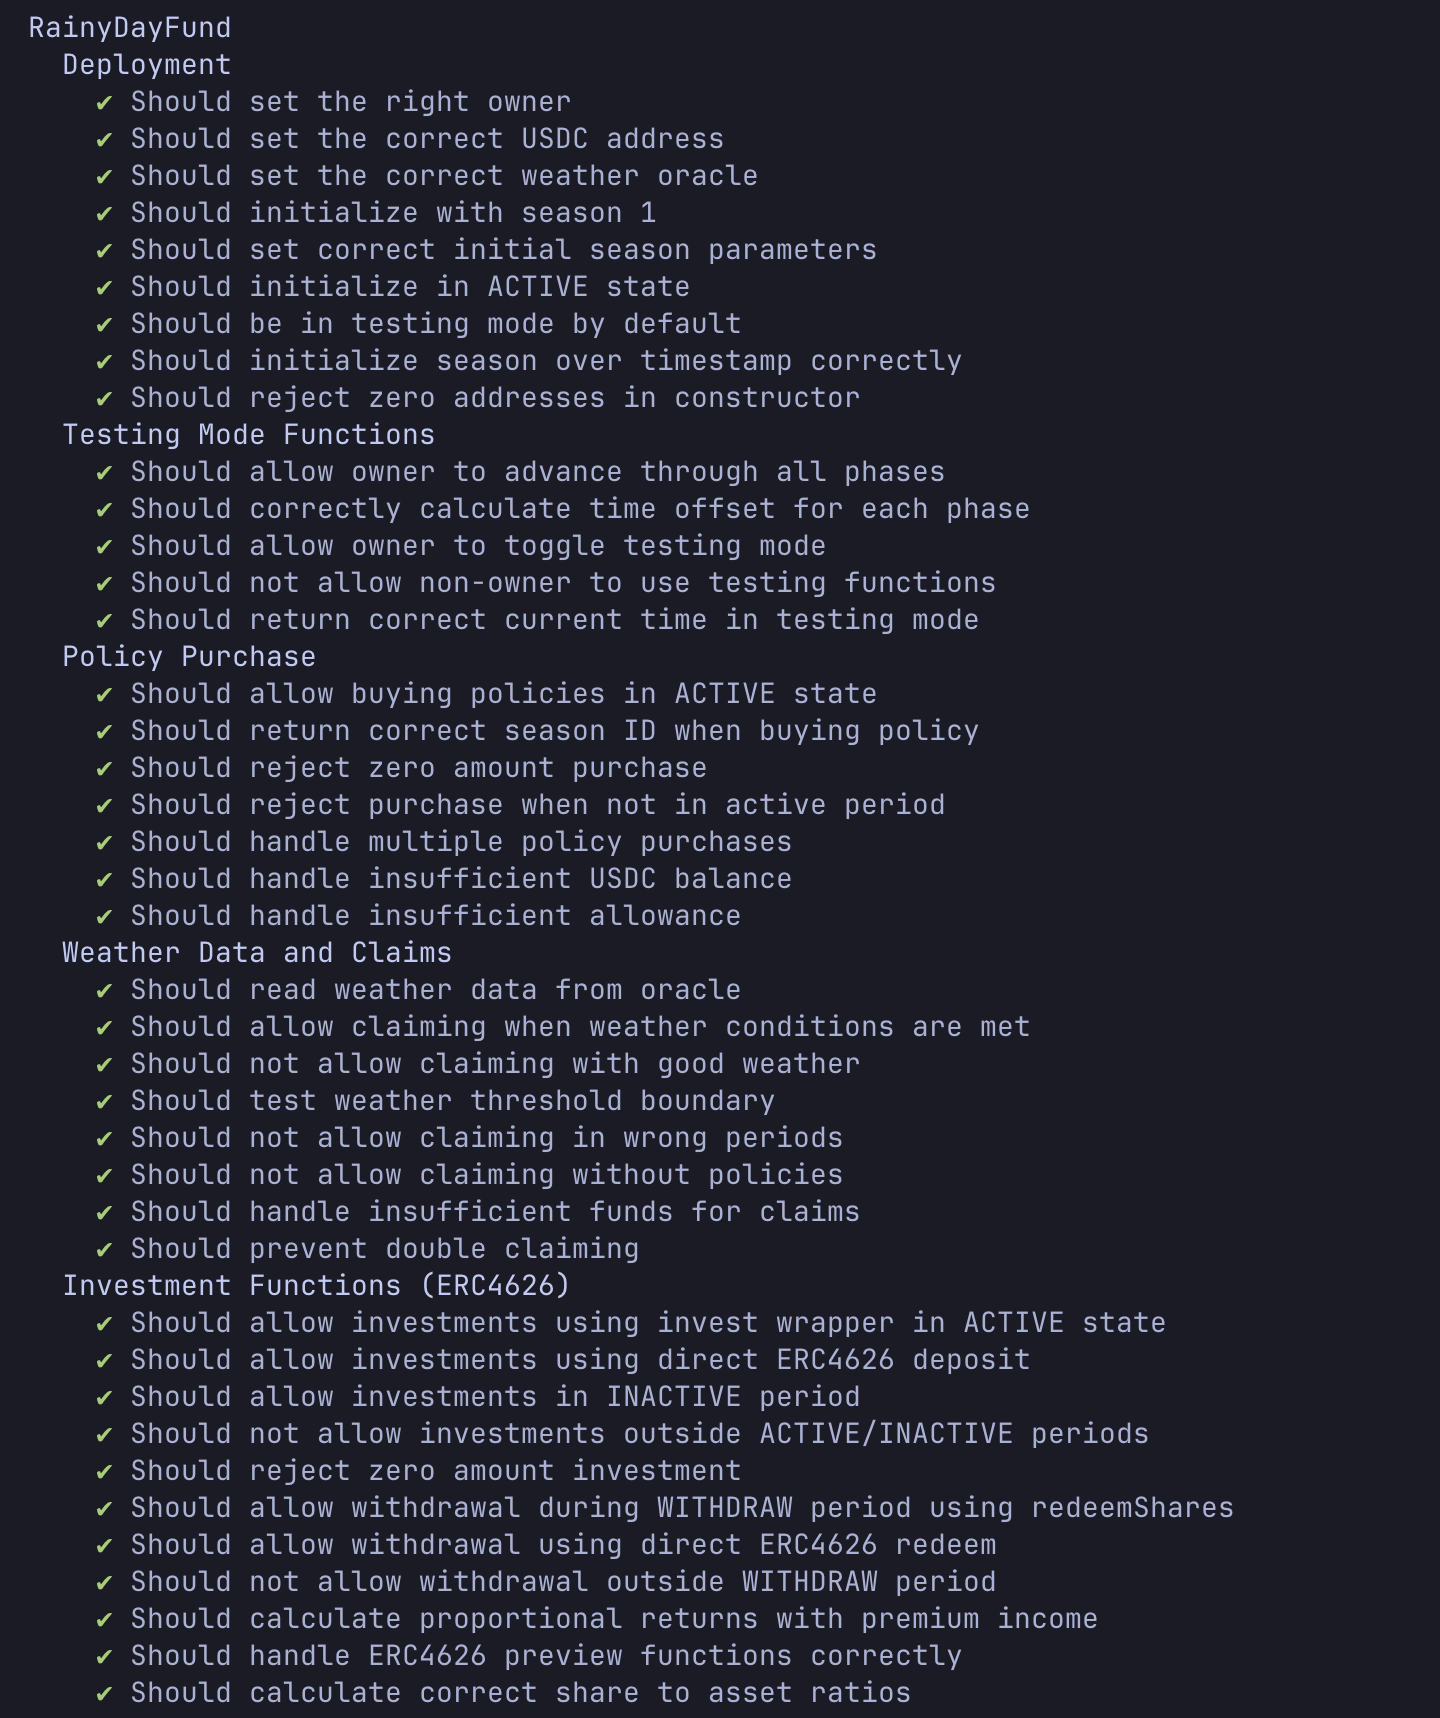
\includegraphics[width=0.95\linewidth]{graphics/Passing_Tests}
			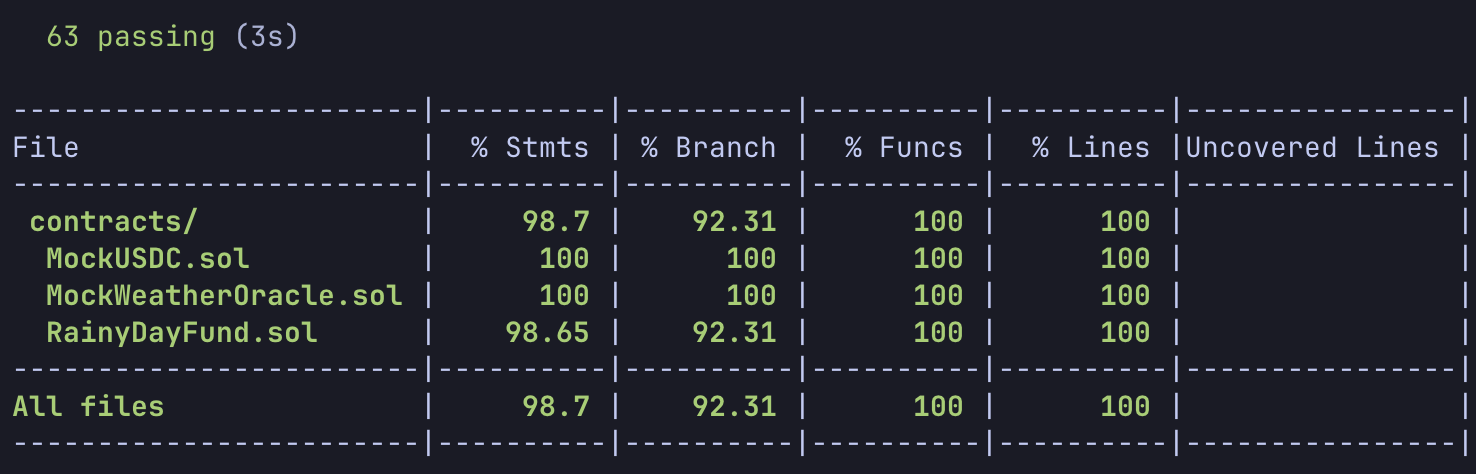
\includegraphics[width=0.95\linewidth]{graphics/Test_Coverage}
			\caption*{(a) Passing Tests and Coverage}
		\end{minipage}\hfill
		\begin{minipage}[b]{0.48\textwidth}
			\centering
			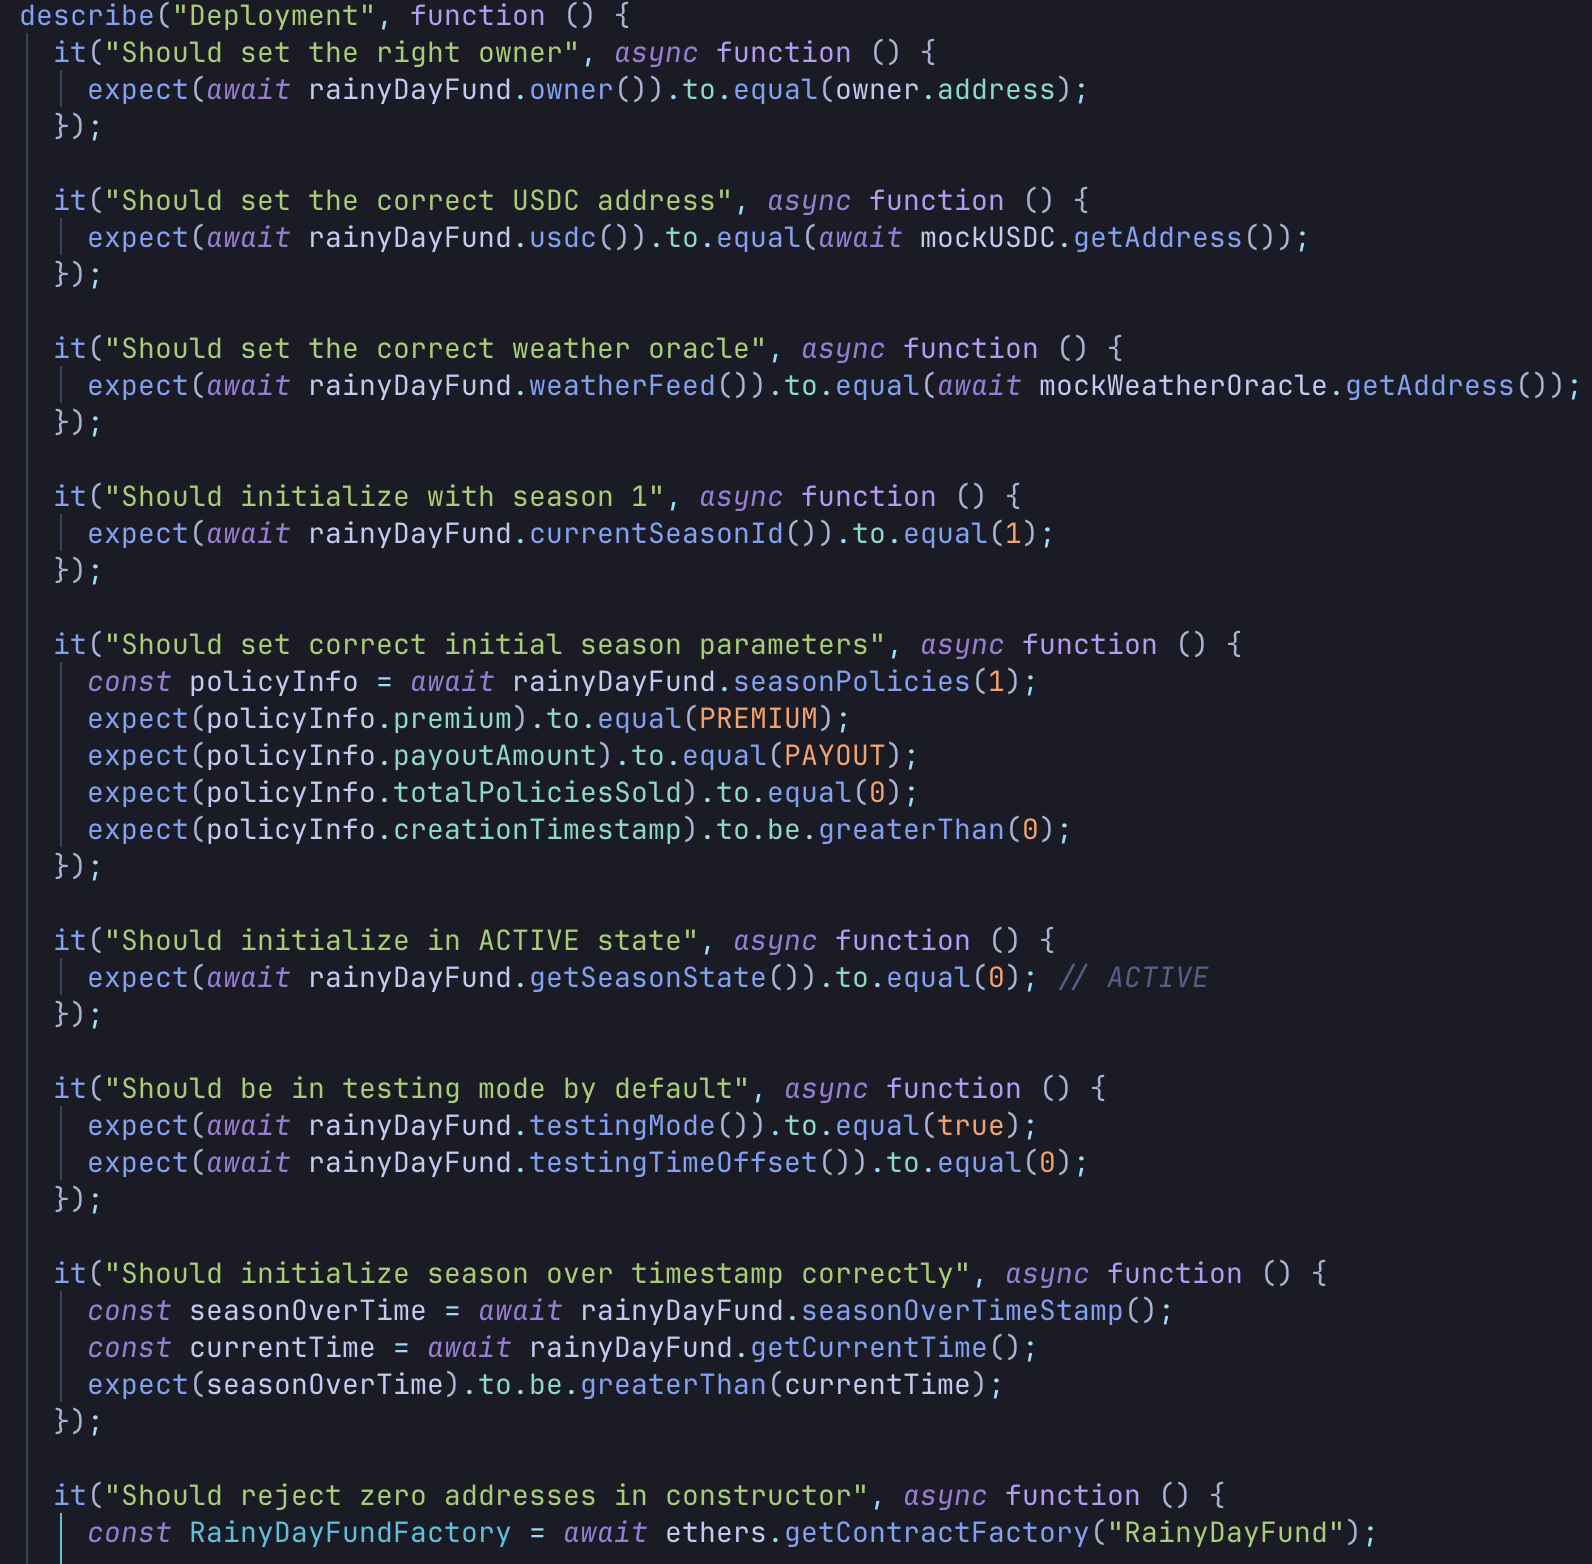
\includegraphics[width=0.95\linewidth]{graphics/Test_Code}
			\caption*{(b) Test Code}
		\end{minipage}
		\caption{Test Setup. (a) Passing tests and coverage; (b) Excerpt of test code. \\ \textit{Source: Author's own.}}
		\label{fig:test-set-up}
	\end{figure}


	\subsection{Outlook \& Next Steps}\label{subsec:outlook}

	The most important next step is integrating real Chainlink oracles for weather data.
	Right now we're using mock data, but production needs reliable, tamper-proof weather information from multiple sources.
	We'll also need to deploy on a real network.
	Layer 2 solutions like Polygon or Arbitrum make sense because gas costs are much lower - important when your users are price-sensitive farmers.
	We might also look into cross-chain deployment to give users more options.
	The smart contract architecture needs some work for production.
	We'll want upgradeability mechanisms so we can fix bugs and add features, but we need to balance that with immutability for user trust.
	Gas optimization is another priority - the current contract works but isn't optimized for cost.
	For additional features, we're thinking about crop-specific insurance products and multi-season coverage.
	The current single-season model is too limiting for real-world agriculture.
	We'd also like to support group policies for farmer cooperatives.
	The frontend needs to be much more user-friendly, especially for people with limited digital experience.
	Mobile-first design is essential since most users will access this through smartphones.
	We'll need offline capabilities too since internet connectivity can be spotty in rural areas.
	Technical priorities include:

	\begin{enumerate}
		\item Chainlink integration for real weather data
		\item Layer 2 deployment for lower costs
		\item Gas optimization and contract upgrades
		\item Mobile-optimized frontend with offline support
		\item Multi-language support and simplified interfaces
	\end{enumerate}

	We're also planning more comprehensive testing on testnets once we sort out the deployment issues.
	The current local testing is good for development, but we need real network conditions to catch problems we haven't thought of.


	\section{Conclusion}\label{sec:conclusion}
	\ldots

    The entire project can be found in the \href{https://github.com/vincentschall/decentralized_weather_insurance}{Github repository}.

	% ---------- Bibliography ----------
	\printbibliography

	\appendix
	\section{Smart Contract Code}\label{sec:contract-code}
		This appendix contains the full source code for the smart contracts implemented in this project.
    These contracts form the core of our decentralized parametric insurance system.

	\subsection{RainyDayFund.sol}\label{subsec:rainy-day-fund}
	The main contract that implements the decentralized parametric insurance system.It handles policy issuance, claims processing, and investment management.

	\begin{lstlisting}[style=soliditystyle, caption={RainyDayFund.sol - Main Insurance Contract},label={lst:lstlistingA}]
    // SPDX-License-Identifier: MIT
    pragma solidity ^0.8.28;

    import "@openzeppelin/contracts/access/Ownable.sol";
    import "@openzeppelin/contracts/utils/ReentrancyGuard.sol";
    import "@openzeppelin/contracts/token/ERC20/ERC20.sol";
    import "@openzeppelin/contracts/token/ERC20/extensions/ERC4626.sol";
    import "@openzeppelin/contracts/token/ERC20/extensions/IERC20Metadata.sol";

    interface AggregatorV3Interface {
      function latestRoundData() external view returns (
        uint80 roundId,
        int256 answer,
        uint256 startedAt,
        uint256 updatedAt,
        uint80 answeredInRound
      );
    }

    contract RainyDayFund is ERC4626, Ownable, ReentrancyGuard {
      IERC20 public immutable usdc;

      uint256 public currentSeasonId;
      uint256 public seasonOverTimeStamp;
      uint256 public constant timeUnit = 30 days;
      uint256 premium = 9 * 10**6; // 9 USDC

      AggregatorV3Interface public weatherFeed;

      // Testing variables for time control
      uint256 public testingTimeOffset;
      bool public testingMode;

      enum SeasonState { ACTIVE, INACTIVE, CLAIM, WITHDRAW, FINISHED }

      struct SeasonPolicy {
        uint256 creationTimestamp;
        uint256 payoutAmount;
        uint256 premium;
        uint256 totalPoliciesSold;
        ERC20 policyToken;
      }

      mapping(uint256 => SeasonPolicy) public seasonPolicies;

      event PolicyBought(address indexed farmer, uint256 seasonId, uint256 amount, uint256 totalPremium);
      event ClaimMade(address indexed farmer, uint256 seasonId, uint256 amount, uint256 totalPayout);
      event InvestmentMade(address indexed investor, uint256 amount);
      event InvestmentWithdrawn(address indexed investor, uint256 amount);
      event NewSeasonStarted(uint256 seasonId, uint256 premium, uint256 payoutAmount);
      event TimeAdvanced(uint256 newTimestamp, SeasonState newState);

      constructor(address _usdcAddress, address _weatherOracle)
      ERC4626(IERC20Metadata(_usdcAddress))
      ERC20("RainyDay Investor Shares", "RDIS")
      Ownable(msg.sender)
      {
        require(_usdcAddress != address(0), "USDC address zero");
        usdc = IERC20(_usdcAddress);

        require(_weatherOracle != address(0), "Weather oracle zero");
        weatherFeed = AggregatorV3Interface(_weatherOracle);

        currentSeasonId = 1;
        _initializeSeason(currentSeasonId);
        seasonOverTimeStamp = getCurrentTime() + 2 * timeUnit;

        // Enable testing mode by default for local testing
        testingMode = true;
      }

      // Testing function to get current time (can be offset in testing mode)
      function getCurrentTime() public view returns (uint256) {
        if (testingMode) {
          return block.timestamp + testingTimeOffset;
        }
        return block.timestamp;
      }

      // Testing function to advance time manually
      function advanceToNextPhase() external onlyOwner {
        require(testingMode, "Not in testing mode");

        SeasonState currentState = getSeasonState();
        uint256 nowBlock = block.timestamp;
        if (currentState == SeasonState.ACTIVE) {
          uint256 target = seasonOverTimeStamp - timeUnit + 1; // +1 to ensure inside the next phase
          testingTimeOffset = target - nowBlock;
        } else if (currentState == SeasonState.INACTIVE) {
          uint256 target = seasonOverTimeStamp + 1;
          testingTimeOffset = target - nowBlock;
        } else if (currentState == SeasonState.CLAIM) {
          uint256 target = seasonOverTimeStamp + timeUnit + 1;
          testingTimeOffset = target - nowBlock;
        } else if (currentState == SeasonState.WITHDRAW) {
          uint256 target = seasonOverTimeStamp + 2 * timeUnit + 1;
          testingTimeOffset = target - nowBlock;
        } else {
          // already finished, do nothing
          emit TimeAdvanced(getCurrentTime(), getSeasonState());
          return;
        }

        emit TimeAdvanced(getCurrentTime(), getSeasonState());
      }

      // Testing function to set testing mode
      function setTestingMode(bool _enabled) external onlyOwner {
        testingMode = _enabled;
        if (!_enabled) {
          testingTimeOffset = 0;
        }
      }

      function _initializeSeason(uint256 seasonId) internal {
        SeasonPolicyToken policyToken = new SeasonPolicyToken(
          string(abi.encodePacked("RainyDay Policy Season ", _toString(seasonId))),
          string(abi.encodePacked("RDP", _toString(seasonId))),
          address(this)
        );

        seasonPolicies[seasonId] = SeasonPolicy({
          creationTimestamp: getCurrentTime(),
          payoutAmount: premium * 4,
          premium: premium,
          totalPoliciesSold: 0,
          policyToken: policyToken
        });

        emit NewSeasonStarted(seasonId, premium, seasonPolicies[seasonId].payoutAmount);
      }

      function getSeasonState() public view returns (SeasonState) {
        uint256 currentTime = getCurrentTime();
        if (currentTime < seasonOverTimeStamp - timeUnit) {
          return SeasonState.ACTIVE;
        } else if (currentTime < seasonOverTimeStamp) {
          return SeasonState.INACTIVE;
        } else if (currentTime < seasonOverTimeStamp + timeUnit) {
          return SeasonState.CLAIM;
        } else if (currentTime < seasonOverTimeStamp + 2 * timeUnit) {
          return SeasonState.WITHDRAW;
        } else {
          return SeasonState.FINISHED;
        }
      }

      modifier onlyAfterFullSeasonCycle() {
        require(getSeasonState() == SeasonState.FINISHED, "Season not fully finished yet");
        _;
      }

      modifier onlyDuringSeason() {
        require(
          getSeasonState() == SeasonState.ACTIVE ||
          getSeasonState() == SeasonState.INACTIVE,
          "Season not active aymore");
          _;
      }

      function startNewSeason(uint256 _premium) external onlyOwner onlyAfterFullSeasonCycle {
        currentSeasonId++;
        premium = _premium;
        seasonOverTimeStamp = getCurrentTime() + 2 * timeUnit;
        _initializeSeason(currentSeasonId);
      }

      function buyPolicy(uint256 _amount) external nonReentrant returns (uint256 seasonId) {
        require(_amount > 0, "Amount > 0");
        require(getSeasonState() == SeasonState.ACTIVE, "Not in active period");

        SeasonPolicy storage policy = seasonPolicies[currentSeasonId];

        uint256 totalPremium = policy.premium * _amount;
        require(usdc.transferFrom(msg.sender, address(this), totalPremium), "Transfer failed");

        SeasonPolicyToken(address(policy.policyToken)).mint(msg.sender, _amount);
        policy.totalPoliciesSold += _amount;

        emit PolicyBought(msg.sender, currentSeasonId, _amount, totalPremium);
        return currentSeasonId;
      }

      function claimPolicies() external nonReentrant {
        require(getSeasonState() == SeasonState.CLAIM, "Not in claim period");

        SeasonPolicy storage policy = seasonPolicies[currentSeasonId];
        SeasonPolicyToken token = SeasonPolicyToken(address(policy.policyToken));
        uint256 amount = token.balanceOf(msg.sender);
        require(amount > 0, "No policies to claim");

        (,int256 weather,) = getWeatherData();
        require(uint256(weather) < 10, "Weather not bad enough");

        uint256 totalPayout = policy.payoutAmount * amount;
        require(usdc.balanceOf(address(this)) >= totalPayout, "Insufficient funds");

        require(usdc.transfer(msg.sender, totalPayout), "Payout failed");
        token.burnFrom(msg.sender, amount);

        emit ClaimMade(msg.sender, currentSeasonId, amount, totalPayout);
      }

      function getWeatherData() public view returns (uint80 roundId, int256 weather, uint256 timestamp) {
        (roundId, weather,,timestamp,) = weatherFeed.latestRoundData();
      }

      // ERC4626 investment logic
      function invest(uint256 assets) external nonReentrant onlyDuringSeason {
        require(assets > 0, "Amount > 0");
        deposit(assets, msg.sender);
        emit InvestmentMade(msg.sender, assets);
      }

      function redeemShares(uint256 shares) external nonReentrant {
        require(getSeasonState() == SeasonState.WITHDRAW, "Not in withdrawal period");
        uint256 assets = redeem(shares, msg.sender, msg.sender);
        emit InvestmentWithdrawn(msg.sender, assets);
      }

      function totalAssets() public view override returns (uint256) {
        return usdc.balanceOf(address(this));
      }

      // minimal utility
      function _toString(uint256 value) internal pure returns (string memory) {
        if (value == 0) return "0";
        uint256 temp = value;
        uint256 digits;
        while (temp != 0) { digits++; temp /= 10; }
        bytes memory buffer = new bytes(digits);
        while (value != 0) { digits--; buffer[digits] = bytes1(uint8(48 + value % 10)); value /= 10; }
        return string(buffer);
      }
    }

    contract SeasonPolicyToken is ERC20 {
      address public immutable rainyDayFund;
      modifier onlyRainyDayFund() { require(msg.sender == rainyDayFund, "Only fund"); _; }

      constructor(string memory name, string memory symbol, address _fund) ERC20(name, symbol) {
        rainyDayFund = _fund;
      }

      function mint(address to, uint256 amount) external onlyRainyDayFund { _mint(to, amount); }
      function burnFrom(address from, uint256 amount) external onlyRainyDayFund { _burn(from, amount); }
    }
    \end{lstlisting}


	\subsection{MockUSDC.sol}\label{subsec:mock-usdc}
	A mock implementation of the USDC stablecoin for testing purposes.
    It implements the ERC20 interface and provides additional minting functionality.

	\begin{lstlisting}[style=soliditystyle, caption={MockUSDC.sol - Mock Stablecoin for Testing},label={lst:lstlisting2}]
    // SPDX-License-Identifier: MIT
    pragma solidity ^0.8.20;

    import "@openzeppelin/contracts/token/ERC20/ERC20.sol";

    contract MockUSDC is ERC20 {
        constructor() ERC20("Mock USDC", "mUSDC") {
            _mint(msg.sender, 1_000_000 * 10 ** decimals());
        }

        function mint(address to, uint256 amount) external {
            _mint(to, amount);
        }
    }
    \end{lstlisting}

	\subsection{MockWeatherOracle.sol}\label{subsec:mock-weather-oracle}
	A mock implementation of a weather data oracle that conforms to Chainlink's AggregatorV3Interface for standardized data feeds. This contract simulates weather data for testing the insurance system.

	\begin{lstlisting}[style=soliditystyle, caption={MockWeatherOracle.sol - Mock Weather Data Oracle},label={lst:lstlisting}]
    // SPDX-License-Identifier: MIT
    pragma solidity ^0.8.28;

    contract MockWeatherOracle {
        int256 public latestWeather;
        uint80 public latestRound;

        constructor(int256 _initialWeather) {
            latestWeather = _initialWeather;
            latestRound = 1;
        }

        function updatePrice(int256 _newWeather) external {
            latestWeather = _newWeather;
            latestRound += 1;
        }

        function latestRoundData()
            external
            view
            returns (
                uint80 roundId,
                int256 answer,
                uint256 startedAt,
                uint256 updatedAt,
                uint80 answeredInRound
            )
        {
            return (
                latestRound,
                latestWeather,
                block.timestamp,
                block.timestamp,
                latestRound
            );
        }
    }
    \end{lstlisting}

	\section{Contract Architecture Analysis}\label{sec:contract-analysis}
	The smart contracts presented above form the foundation of our decentralized parametric insurance system.
    Each plays a specific role in the ecosystem:

	\subsection{RainyDayFund}\label{subsec:analysis-rainy-day-fund}
	This is the core contract of the system and implements several key components:

	\begin{enumerate}
	    \item \textbf{Policy Management}: Handles the issuance of policy tokens to farmers and tracks active policies.
	    \item \textbf{Season States}: Implements a state machine for managing different phases of the insurance season (active, inactive, claim, withdraw, finished).
	    \item \textbf{Claims Processing}: Processes claims by verifying policy ownership and weather conditions.
	    \item \textbf{Investment Management}: Allows investors to provide liquidity to the risk pool and earn returns.
	    \item \textbf{Weather Data Integration}: Interfaces with the weather oracle to retrieve data for claims verification.
	\end{enumerate}

	The contract employs several important design patterns:
	\begin{itemize}
	    \item \textbf{ERC4626 Tokenized Vault}: For managing investments and yield generation.
	    \item \textbf{ERC20 Policy Tokens}: For representing insurance policies as transferable assets.
	    \item \textbf{Non-reentrant Guards}: To prevent reentrancy attacks during financial transactions.
	    \item \textbf{Owner Controls}: To manage system parameters and seasonal transitions.
	    \item \textbf{State Machine}: To enforce the correct sequence of operations based on the current season state.
	\end{itemize}

	\subsection{MockUSDC}\label{subsec:analysis-mock-usdc}
	This contract simulates a stablecoin for testing purposes.
    In a production environment, this would be replaced with a real stablecoin like USDC. The mock implementation provides:

	\begin{itemize}
	    \item Standard ERC20 functionality for token transfers and allowances
	    \item Additional minting capability for testing purposes
	    \item Initial supply of 1,000,000 tokens for the contract deployer
	\end{itemize}

	\subsection{MockWeatherOracle}\label{subsec:analysis-mock-weather-oracle}
	This contract simulates a weather data oracle, conforming to Chainlink's AggregatorV3Interface standard.
    In production, this would be replaced with actual Chainlink oracles providing real weather data.
    The mock implementation provides:

	\begin{itemize}
	    \item Storage for weather data values
	    \item Functions to update weather data (for testing purposes)
	    \item Standard interface conformance to ensure compatibility with the main contract
	\end{itemize}

\end{document}
